\section{Hypothesis and Objective Validation}
\label{sec:conclusions:hypothesis}

In the beginning of this dissertation, concretely in Section \ref{sec:intro:hypothesis}, a hypothesis was posed, which stated the following:

\vspace{0.5cm}

\noindent\fbox{
    \parbox{\textwidth}{
    \begin{hypo}
Using domain experts' previous knowledge as generic but incomplete activity models and data-driven learning techniques on user generated data, it is possible to learn accurately new actions to obtain personalised activity models for every user. 
\end{hypo}
}
}

\vspace{0.5cm}

In order to be able to validate this hypothesis, a goal was also defined, which is also shown below for convenience:

\vspace{0.5cm}

\noindent\fbox{
    \parbox{\textwidth}{
\begin{goal}
To design and implement a learning system that uses generic but incomplete activity models to analyse unlabelled activity sensor datasets and acquire personalised models which contain new actions.
\end{goal}
}
}

\vspace{0.5cm}

To achieve such a goal, some specific and measurable objectives were identified in Section \ref{sec:intro:hypothesis}. It is the moment now to go through all those objectives and see whether they have been addressed in this dissertation. 

\begin{enumerate}
 \item \textit{To study the current state of the art on knowledge- and data-driven activity modelling and recognition.} Chapter \ref{cha:soa} provides a deep and critical study of the current state of the art, analysing activity monitoring, modelling and recognition. Special attention has been paid to activity modelling, presenting data-driven, knowledge-driven and even hybrid approaches and identifying their advantages and disadvantages.
 \item \textit{To choose a knowledge representation formalism and design proper structures to represent domain experts' knowledge.} This objective has been addressed in Chapter \ref{cha:archi}. A light-weight knowledge representation formalism has been chosen, namely the JavaScript Object Notation framework (JSON). Using JSON, the context knowledge file shows structures to represent activities, objects and sensors.
 \item \textit{To design and implement a multiple step learning algorithm which uses previous knowledge and user generated data to obtain personalised activity models.} The design of the learning system and its inspiration have been presented in Chapter \ref{cha:archi}. Moreover, implementation details of the system architecture have been provided, showing samples of the used files. The modules identified in the architecture, which constitute the multiple step learning process have been explained in the following chapters: Chapter \ref{cha:clustering} introduces the activity clustering process and Chapter \ref{cha:learner} describes in detail the activity model learner algorithm. All the implementation work has been done using Python 2.7.
 \item \textit{To identify the evaluation methodology for the learning system which better addresses the requirements of the system.} Chapter \ref{cha:evaluation} analyses the so-called standard methodology for activity modelling and recognition. It is concluded that using the standard methodology is not feasible to properly validate the learning system. In consequence, a novel hybrid methodology is developed and presented in Section \ref{subsec:evaluation:hybrid}, which combines real users' inputs and a simulator. 
 \item \textit{To validate the obtained results quantitatively, with the objective of capturing the 100\% of real activity models performed by a user.} The results of several experiments are presented in Chapter \ref{cha:evaluation}. It has been shown that the 100\% of action sequences executed by several users to perform the same seven activities are captured and modelled (Section \ref{subsubsec:evaluation:eam:results}). These results are obtained in scenarios which contain high levels of sensor noise. 
\end{enumerate}


For the sake of clarity, Figure \ref{fig-obj-contr-chap} provides a diagram where the objectives, the contributions that are related to these objectives and their location in this dissertation are shown.

\begin{figure}[htbp]
\centering
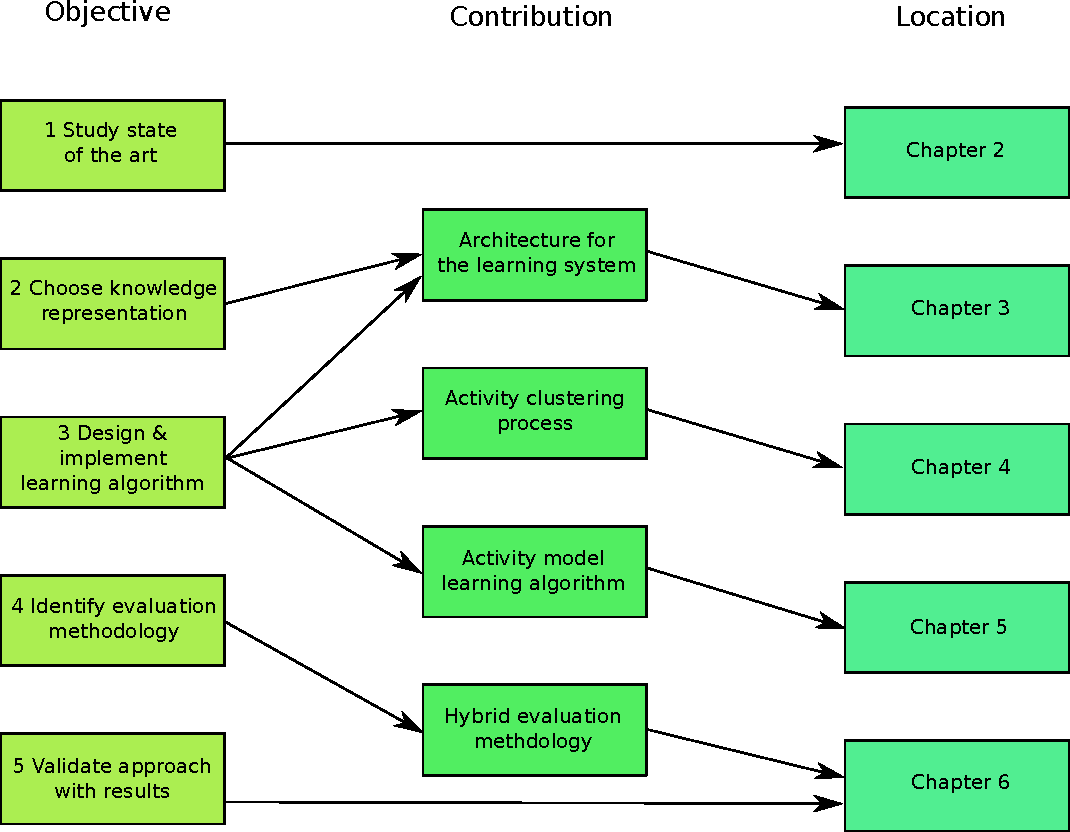
\includegraphics[width=\textwidth]{obj-contr-chap.pdf}
    \caption{The relation of the objectives defined in Section \ref{sec:intro:hypothesis}, the contributions listed in Section \ref{sec:conclusions:contrib} and their location in this dissertation.}
    \label{fig-obj-contr-chap}
\end{figure}

It can be claimed that all the objectives set in Section \ref{sec:intro:hypothesis} have been accomplished in this dissertation. As a consequence of this, the goal of the dissertation has been achieved. The EAM learning system which is composed by the activity clustering process (Chapter \ref{cha:clustering}) and the activity model learner (Chapter \ref{cha:learner}) has been implemented and tested. The learning system uses generic but incomplete activity models and unlabelled sensor datasets. As a result of the learning process, personalised activity models have been shown to be learnt, capturing personal ways of performing activities in terms of actions.

Finally, through the accomplishment of the objectives and the goal, the hypothesis of this dissertation has been validated. The results obtained in Chapter \ref{cha:evaluation} proof that it is possible to learn accurately new actions to obtain personalised activity models for every user, combining generic but incomplete activity models and data-driven learning techniques. Section \ref{subsubsec:evaluation:eam:results} shows the results that proof that all the actions executed by several users to perform different activities are accurately captured and modelled. Several spurious models are also learnt in the process, but the number of such models is assumable as discussed in Section \ref{subsubsec:evaluation:eam:discussion}.